\section{Trigonometric Functions}
\label{sec:trig}

Most applied calculus texts skip {\bf trigonometric}\index{Functions!trigonometric} functions, but they are extremely powerful for modeling periodic or seasonal data. We will keep the treatment of these models very basic and intuitive, but independent from the rest of the text; it is optional. For the scientist, trigonometric functions are indispensable. However, for our purposes, we will focus our attention exclusively on two related functions: the {\bf sine}\index{Function!sine} and {\bf cosine}\index{Function!cosine} functions.

\subsection{Definitions}

% Insert definitions with graphs here.

A {\bf sine wave}\index{Sine wave} is of the form
\begin{equation}
\label{eq:sine}
f(x) = v + a \cdot \sin\left(\frac{2\pi(x-h)}{p}\right) \enspace .
\end{equation}
where $v$ is the {\bf vertical shift}\index{Shift!vertical} (mean of the data), $a$ is the {\bf amplitude}\index{Amplitude} of the wave (roughly the difference between the maximum and the mean of the data), $h$ is the {\bf horizontal shift}\index{Shift!horizontal} (where the data is at the mean and begins to rise to the maximum), and $p$ is the {\bf period}.

\subsection{Modeling with Sine Waves}

Consider the following table that we saw in Sections \ref{sec:models} and \ref{sec:polynomial} on the fuel oil usage of Plant W in 2016. One task that we were unable to complete before was to determine a model that would reflect the seasonality of the data. In other words, since the data represents a calendar year, we want a model that will oscillate and finish at the same output value as the output value of the beginning point. A {\bf trigonometric model}\index{Model!trigonometric} serves that very purpose.

\begin{table}[!ht]
\centering
\begin{tabular}{l*{12}{c}}
\toprule
Month & Jan. & Feb. & Mar. & Apr. & May & June & July & Aug. & Sep. & Oct. & Nov. & Dec. \\
\midrule
Oil (gal) & 573.0 & 850.0 &  425.3 & 800.1  & 818.9 &  880.9 &  296.5 & 198.7 & 105.4 & 72.0 & ?? & 638.0\\
\bottomrule
\end{tabular}
\caption{Fuel Oil Usage at Plant W in 2016}
\label{tab:1-9-oil}
\end{table}

Given our data, we don't know the vertical shift, the amplitude, or the horizontal shift, but we do know the period. Since the input is in months and there are 12 months in a year, we choose $p = 12$ from \ref{eq:sine}. We then fit a sine wave to the data and get the following model.

If $m$ is the $m$th month of the year, then Plant W burned oil at a rate of
$$f(m) = 492.82 - 334.33\sin\left(\frac{2\pi(m+29.49)}{12} \right) \mbox{ gallons per month}$$
in 2016.

Graphing $y=f(m)$ with the scatter plot of Table \ref{tab:1-9-oil} gives us the following plot to verify that the model makes sense.
\begin{figure}[!ht]
%\begin{wrapfigure}{R}{0.3\textwidth}
    \centering
    %\vspace{-20pt}
    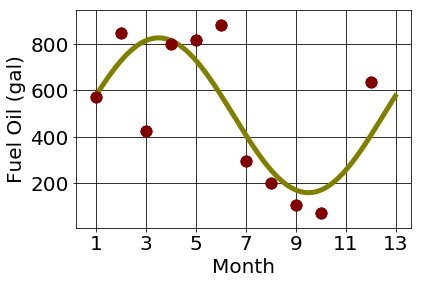
\includegraphics[width=0.3\textwidth]{img/chap1/sec1-9/fig1-9-oil-curve.png}\\
    \caption{Fuel Oil Usage by Plant W in 2016 Fitted by a Sine Wave.}
    \label{fig:1-9-oil-curve}
%    \vspace{-20pt}
%\end{wrapfigure}
\end{figure}
